\chapter{Secure Perfect Connected Domination in Graphs}
\noindent
In this chapter, we have introduced another variant of secure domination named as secure perfect connected domination. We investigated bounds on minimum secure perfect connected domination and for some basic classes of graphs we obtained exact value of it . 
\section{Secure Perfect Connected Dominating Set}
\noindent
%\newtheorem{Definition}{Definition}
\begin{Definition}
A secure perfect connected dominating set (SPCDS) of a graph $G=(V,E)$ is a subset of vertices where $G[S]$ is connected and $\forall v \in V(G)\setminus S$, a unique vertex $u \in S$ exists such that $u$ and $v$ are adjacent in $G$ and the set $(S\setminus \lbrace u \rbrace) \cup \lbrace v \rbrace$ is a CDS of $G$.  
\end{Definition}
\noindent The \textit{secure perfect connected domination number} of $G$ is defined as the minimum cardinality of a SPCDS and is denoted by $\gamma_{spc}(G)$.\\
Since every SPCDS is a PSDS and every PSDS is a SDS, the inequality $\gamma_{spc}(G) \geq \gamma_{ps}(G) \geq \gamma_s(G)$ holds for every connected graph $G$.
\begin{Definition}
Let $S$ be a SPCDS of a graph $G$. If $\forall v \in V(G) \setminus S$ a unique vertex $u \in S$ exists in $G$ such that the set $(S\setminus \lbrace u \rbrace) \cup \lbrace v \rbrace$ is a CDS of $G$, then we say that $u$ S-defends $v$ or $v$ is S-defended by $u$ or simply $u$ defends $v$ or $v$ is defended by $u$ if the context is clear.
\end{Definition}
%\newtheorem{proposition}{Proposition}
\section{Some Results on Secure Perfect Connected Domination}
\begin{proposition}
For $n \geq 3$ of a connected graph $G$, let $S$ be a SPCDS then:
\end{proposition}
\noindent (i.) \textit{Each cut-vertex is in $S$\\}
(ii.) \textit{Each pendant vertex is in $S$\\}
(iii.) \textit{If $G$ has a pair of non-adjacent vertices then $\gamma_{spc}(G) \geq 3$}.
\begin{proof}
(i.) Assume a cut-vertex $u$ in $G$. By contradiction, assume $u \notin S$. Since $G\setminus \lbrace u \rbrace$ is divided into two or more connected components and to dominate vertices in each component at least one vertex from each component must be in $S$. In this case $G[S]$ is not connected, which is a contradiction. Hence $u$ must be in $S$.\\
(ii.) Let $u$ be a pendant vertex in $G$. By contradiction, assume $u \notin S$. Let $v$ be a neighbor of $u$, clearly $v$ is a cut-vertex. From (i), vertex $v \in S$ and $(S\setminus \lbrace v \rbrace ) \cup \lbrace u \rbrace$ becomes disconnected, which is a contradiction. Hence $u$ must be in $S$.\\
(iii.) Let the vertices $\{u,v\} \in V(G)$ and the edge $(u,v) \notin E(G)$. By contradiction, assume that $\gamma_{spc}(G) < 3$. Then consider the following cases:\\
\textit{Case }1: If $\gamma_{spc}(G) = 1$. Consider $S= \{ x \}$ be a SPCDS in $G$ with $|S|=1$, then $(u,x),(v,x) \in E(G)$ and  $(S\setminus \lbrace x \rbrace) \cup \lbrace u \rbrace$ is not a DS in $G$, which is a contradiction.\\
\textit{Case }2: If $\gamma_{spc}(G) = 2$. Consider $S=\{ x,y \}$ be a SPCDS of $G$ with $|S|=\gamma_{spc}(G)$ then $ (v,y),(u,x) \in E(G)$ and $(S\setminus \lbrace y \rbrace ) \cup \lbrace v \rbrace$, $(S\setminus \lbrace x \rbrace ) \cup \lbrace u \rbrace$ is not connected, which is a contradiction.\\ Hence from case 1 and case 2, $\gamma_{spc}(G) \geq 3$.
\end{proof}
\begin{proposition}
Let $G$ be a connected graph. Then $\gamma_{spc}(G)=1$ if and only if $G$ is a complete graph.  
\end{proposition}
\begin{proof}
For a graph $G$ let $S$ be a SPCDS with $|S|=1$. By contradiction, assume $G$ is not a complete graph. There exists at least a pair of vertices which are not adjacent in $G$. From proposition 4.2.1, $\gamma_{spc}(G) \geq 3$, which is a contradiction. Conversely, let $G$ be a complete graph and by contradiction, assume $S$ be a SPCDS of $G$ with $|S| \geq 2 $. Then $\forall x \in V(G)\setminus S$ there exists at least two vertices which defends, which is a contradiction. Hence $\gamma_{spc}(G)=1$ if and only if $G$ is a complete graph.
\end{proof}
\begin{proposition}
Let $G$ be a connected graph with $n$ number of vertices, which is not complete, $\gamma_{spc}(G)=n$ if $G$ has at least two vertices $u$ and $v$ of degree $n-1$.
\end{proposition}  
\begin{proof}
For a graph $G$ let $S$ be a SPCDS. Since $G$ is not complete, by proposition 4.2.2, $\gamma_{spc}(G) \geq 2$. By contradiction, assume $|S| \leq n-1$. Then consider the following cases:\\
\textit{Case }1 : If $u,v \notin S$. Vertices $u$ and $v$ are defended by at least two vertices of $S$, which is a contradiction.\\
\textit{Case }2 : If $u \in S$ and $v \notin S$. Vertex $v$ is defended by at least two vertices of $S$, which is a contradiction.\\
\textit{Case }3 : If $u \notin S$ and $v \in S$. Same as case 2.\\
\textit{Case }4 : If $u ,v \in S$. Each vertex $w \in V(G)\setminus S$ is defended by both the vertices $u$ and $v$, which is a contradiction.\\
Hence $\gamma_{spc}(G)=n$.
\end{proof}
\begin{proposition}
Removal of an edge $e$ from a graph $G$, increases $\gamma_{spc}(G \setminus \lbrace e \rbrace)$ arbitrarily.
\end{proposition}
\begin{proof}
Let $G \cong K_n$, where $n \geq 4$. By proposition 4.2.2, $\gamma_{spc}(K_n) = 1$ and by proposition 4.2.3, $\gamma_{spc}(K_n \setminus \lbrace e \rbrace) = n$. Hence the result.
\end{proof}
\begin{proposition}
Removal of a vertex $v$ from a graph $G$, increases $\gamma_{spc}(G\setminus \lbrace v \rbrace)$ arbitrarily.
\end{proposition}
\begin{proof}
Consider the following graph $G$ and let a SPCDS of $G$ be $S = \lbrace a,b,c \rbrace$. Hence $\gamma_{spc}(G) \leq 3$. If we remove a vertex $c$ from $G$, then SPCDS of the graph $G\setminus \lbrace c \rbrace$ is $\lbrace a,v_1,v_2,...,v_l,b \rbrace$ i.e. $\gamma_{spc}(G\setminus \lbrace c \rbrace)\leq l+2$.\\
\begin{figure}[H]
\centering
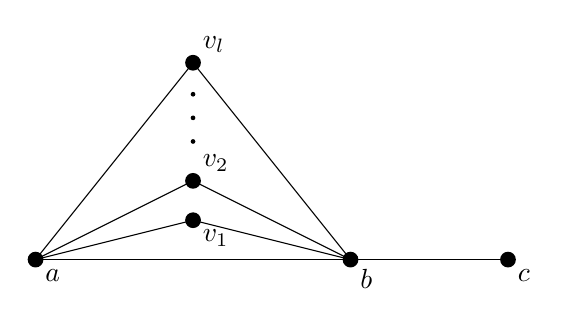
\begin{tikzpicture}
\draw (0,1) -- (4,1);
\draw (4,1) -- (6,1);
\draw (0,1) -- (2,1.5);
\draw (4,1) -- (2,1.5);
\draw (0,1) -- (2,2);
\draw (4,1) -- (2,2);
\draw (0,1) -- (2,3.5);
\draw (4,1) -- (2,3.5);

\fill (0,1) circle(0.1cm) node[anchor=north west] {$a$};
\fill (4,1) circle(0.1cm) node[anchor=north west] {$b$};
\fill (6,1) circle(0.1cm) node[anchor=north west] {$c$};
\fill (2,1.5) circle(0.1cm) node[anchor=north west] {$v_1$};
\fill (2,2) circle(0.1cm) node[anchor=south west] {$v_2$};
\fill (2,3.5) circle(0.1cm) node[anchor=south west] {$v_l$};
\fill (2,2.5) circle(0.3mm);
\fill (2,2.8) circle(0.3mm);
\fill (2,3.1) circle(0.3mm);

\end{tikzpicture}
\caption{Graph $G$}
\end{figure}
\end{proof}

\begin{proposition}
The following results hold:
\end{proposition}
\noindent (i.) For $n \geq 3$, let $T$ be a tree,  $\gamma_{spc}(T)=n$\\
(ii.) For $n \geq 4$, let $C_n$ be a cycle,  $\gamma_{spc}(C_n)=n$\\
(iii.) For $r,s \geq 2$, let $K_{r,s}$ be a complete bipartite graph,   $\gamma_{spc}(K_{r,s})=r+s$\\
(iv.) For $p,q \geq 2$, let $Wd_{p,q}$ be a windmill graph,  $\gamma_{spc}(Wd_{p,q})=q+1$.
\begin{proof}
(i.) In a tree $T$, either a vertex is a cut-vertex or a pendant vertex. Hence by proposition 4.2.1, $\gamma_{spc}(T)=n$.\\
(ii.) By contradiction, assume  $\gamma_{spc}(C_n) < n$. Let $S$ be a SPCDS of $C_n$, with $|S| < n$. And let $u$ be a vertex of $C_n$ and $v,w$ be its neighbors. If $u \notin S$, then to dominate $u$ either $v$ or $w$ or both must be in $S$. Now consider the following cases:\\
\textit{Case }1: $v,w \in S$. Clearly $|S| \leq n-1$. But vertex $u$ is defended by $v~ \&~ w$, which is a contradiction.\\
\textit{Case }2: $v\in S$ and $w \notin S$. Clearly $|S| \leq n-2$. But $(S\setminus \lbrace v \rbrace) \cup \lbrace u \rbrace$ becomes disconnected, which is a contradiction.\\
\textit{Case }3: $v \notin S$ and $w \in S$. Same as case 2.\\
Hence $\gamma_{spc}(C_n) = n$.\\
(iii.) Let $X = \lbrace x_1,x_2,...,x_r\rbrace $ and $Y=\lbrace y_1,y_2,...,y_s \rbrace $ be the bipartition of $K_{r,s}$. By contradiction, assume $\gamma_{spc}(K_{r,s}) < r+s$. Let $S$ be a SPCDS of $K_{r,s}$ with $|S| < r+s$. Then consider the following cases:\\
\textit{Case }1: $|S \cap X| < |X|$. In this case, some vertex $x$ exists in $G$ such that $x \in X$, $x \notin S$ and is defended by all the vertices of $S \cap Y$, which is a contradiction.\\
\textit{Case }2: $|S \cap Y| < |Y|$. Same as case 1.\\
Hence $\gamma_{spc}(K_{r,s}) = r+s$.\\
(iv.) Let $G \cong Wd_{p,q}$ and $v_c$ be the common center vertex. Since $v_c$ is a cut-vertex, by proposition 4.2.1, $v_c$ is part of every SPCDS of $G$. Clearly, $\gamma_{spc}(G) \geq q+1$, as there are $q$ connected components in $G \setminus \lbrace v_c \rbrace$. It can be easily to verify that a vertex from each connected component of $G \setminus \{ v_c \}$ and a set which contains $v_c$ is a SPCDS of $G$. Hence $\gamma_{spc}(G) \leq q+1$. Therefore $\gamma_{spc}(Wd_{p,q})=q+1$.
\end{proof}
\noindent The following corollary follows from statement (i) of Proposition 4.2.1.
\newtheorem{Corly}{Corollary}
\begin{Corly}
Let $P$ be a path with $n \geq 3$, then $\gamma_{spc}(p)=n$.
\end{Corly}

\begin{proposition}
Let $k,n$ be two non-negative integers and $W_n$ be a wheel graph with $n \geq 7$ vertices, then
\[
\gamma_{spc}(W_n) = \begin{cases}
k+1, & \text{for }n=3k+1 \\
k+2, & \text{for }n=3k+2 \\
k+3, & \text{for }n=3k+3. \\
\end{cases} 
\]
\end{proposition}
\begin{proof}
The vertices of $W_n$ are labeled as $V(W_n)= \{ v_1, v_2,...,v_n\}$ such that $v_1, v_2,...,v_{n-1}$ is a cycle of length $n-1$. Let
\[
S = \begin{cases}
\lbrace v_{3i+1}:0\leq i < k \rbrace \cup \lbrace v_{3k+1} \rbrace, & \text{if }n=3k+1 \\
\lbrace v_{3i+1}:0\leq i < k \rbrace \cup \lbrace v_{3k+1},v_{3k+2} \rbrace, & \text{if }n=3k+2 \\
\lbrace v_{3i+1}:0\leq i < k \rbrace \cup \lbrace v_{3k+1},v_{3k+2},v_{3k+3} \rbrace, & \text{if }n=3k+3. \\
\end{cases} 
\]
Clearly $S$ is a CDS of $W_n$. For every vertex $u \in S \setminus V(W_n)$, there exists a unique vertex $v \in S$ such that $(S \setminus \lbrace v \rbrace) \cup \lbrace u \rbrace$ is a CDS of $W_n$. Hence $S$ is a SPCDS of $W_n$ and $\gamma_{spc}(W_n) \leq |S|$.\\
The following claim is useful in proving the lower bound.\\
\textbf{Claim} : $v_n$ is part of every SPCDS of $W_n$.\\
\textit{Proof of claim} : By contradiction, assume $S$ be a SPCDS of $W_n$ and $v_n \notin S$. Since $n \geq 7$, $|S \cap \lbrace v_1, v_2, ... , v_{n-1} \rbrace | \geq 2$ and so there exists at least two vertices by which $v_n$ is defended, which contradicts our assumption that $S$ is a SPCDS of $W_n$. Hence $v_n \in S$. \\
Next we show that $\gamma_{spc}(W_n) \geq k+3$ if $n \geq 7 $ and $n=3k+3$. \\
By contradiction, assume that $\gamma_{spc}(W_n) < k+3$. Since $v_n$ is part of every SPCDS of $W_n$, $| \lbrace v_1,v_2,...,v_{n-1} \rbrace \cap S | < k+2$. Now, there exists two vertices $v_i,v_j \in S \cap \lbrace v_1,v_2,..., v_{n-1} \rbrace $, such that $( v_{i+1},...,v_{j-1}) \cap S = \phi$ and $j-i > 3$ or $j-i=2$. If $j-i=2$, then vertex $v_{i+1}$ is defended by two of its neighbors, which is a contradiction. If $j-i > 3$, then $ v_{i+2}$ is dominated by only $v_n$ but $(S\setminus \lbrace v_n \rbrace) \cup \lbrace v_{i+2} \rbrace$ is not connected, a contradiction. Hence $\gamma_{spc}(W_n) \geq k+3$. Therefore $\gamma_{spc}(W_n) = k+3$, if $n=3k+3$. Similarly we can prove for $n=3k+1$ and $n=3k+2$.
\end{proof}

\begin{proposition}
Let $k,n$ be two non-negative integers and $F_n$ be the fan graph with $n \geq 5$ vertices, then 
\[
\gamma_{spc}(F_n) = \begin{cases}
k+2, & \text{for }n=3k+2 \\
k+3, & \text{for }n=3k+3 \\
k+4, & \text{for }n=3k+4. \\
\end{cases} 
\]
\end{proposition}
\begin{proof}
The vertices of $F_n$ are labeled as $V(F_n)= \{ v_1, v_2,...,v_n\}$ such that $v_1, v_2,...,v_{n-1}$ is a path of length $n-1$.  Let
\[
S = \begin{cases}
\lbrace v_{3i+1}:0\leq i < k \rbrace \cup \lbrace v_{3k+1},v_{3k+2} \rbrace, & \text{if }n=3k+2 \\
\lbrace v_{3i+1}:0\leq i < k \rbrace \cup \lbrace v_{3k+1},v_{3k+2},v_{3k+3} \rbrace, & \text{if }n=3k+3 \\
\lbrace v_{3i+1}:0\leq i < k \rbrace \cup \lbrace v_{3k+1},v_{3k+2},v_{3k+3},v_{3k+4} \rbrace, & \text{if }n=3k+4. \\
\end{cases} 
\]
Clearly $S$ is a SPCDS of $F_n$ and $\gamma_{spc}(F_n) \leq |S|$. With similar argument given in proposition 4.2.7, we can prove that $\gamma_{spc}(F_n) \geq |S|$. Hence the result.
\end{proof}